\documentclass[14pt,c]{beamer}

\usecolortheme{owl}
\setbeamercolor{frametitle}{bg=black}
\setbeamertemplate{frametitle}[default][center]
\setbeamertemplate{caption}[numbered]
\setbeamertemplate{caption label separator}{: }
\setbeamercolor{caption name}{fg=normal text.fg}
% \beamertemplatenavigationsymbolsempty%
\addtobeamertemplate{navigation symbols}{}{%
    \usebeamerfont{footline}%
    \usebeamercolor[white]{footline}%
    \hspace{1em}%
    \insertframenumber/\inserttotalframenumber%
}

\usepackage{biblatex}
\addbibresource{references.bib}
\renewcommand*{\bibfont}{\footnotesize}

% Fonts
\usefonttheme{professionalfonts} % So beamer won't change fonts
\usepackage{fontspec}
\setmainfont[Numbers={Lining,OldStyle}]{Linux Libertine}
\setsansfont{Linux Biolinum}
\usepackage[small,euler-digits]{eulervm} % For beamer slides
% \usepackage[libertine,vvarbb]{newtxmath}
\usepackage{realscripts}
\usepackage[scr=esstix,cal=boondoxo]{mathalfa}
\usepackage{bm} % Load after math font configuration
\setmonofont[Scale=MatchLowercase]{Iosevka}

% use microtype if available
\IfFileExists{microtype.sty}{\usepackage{microtype}}{}
\hypersetup{%
            pdftitle={Towards the entropy of images},
            pdfauthor={Alex Striff},
            pdfborder={0 0 0},
            breaklinks=true}
\urlstyle{same} % don't use monospace font for urls

% \setlength{\parindent}{0pt}
% \setlength{\parskip}{6pt plus 2pt minus 1pt}
% \setlength{\emergencystretch}{3em}  % prevent overfull lines
\providecommand{\tightlist}{%
  \setlength{\itemsep}{0pt}\setlength{\parskip}{0pt}}
\setcounter{secnumdepth}{0}

\usepackage{physics}
\usepackage{siunitx}
\usepackage{tikz}
\usetikzlibrary{arrows}
\tikzset{% Animate with beamer overlays
  invisible/.style={opacity=0},
  visible on/.style={alt={#1{}{invisible}}},
  alt/.code args={<#1>#2#3}{%
    \alt<#1>{\pgfkeysalso{#2}}{\pgfkeysalso{#3}} % \pgfkeysalso doesn't change the path
  },
}

\graphicspath{{./figs/}}

\title{Towards the entropy of images}
\subtitle{Pictures in less than a thousand words}
% \subtitle{\textsc{Nsf} \textsc{rpi} \textsc{reu} midterm presentation}
\author{Alex Striff \\ Advisor: Vincent Meunier}
\institute{Reed College}
\date{July 10, 2020}

\begin{document}
\frame{\titlepage}

\begin{frame}{Outline}
  \begin{itemize}
    \item What are we after?
    \item Information theory
    \item The maximum entropy method
    \item Toy models of image fluctuation
    \item The Wang-Landau algorithm
    \item Next steps
  \end{itemize}
\end{frame}

\begin{frame}
  Information from a random variable $X$ being $x \in \mathcal{X}$?
  \onslide<+->
  \begin{itemize}
    \item<+-> If $P(x) = 1$, $I(x) = 0$
    \item<+-> If $P(x) < P(x')$, $I(x) > I(x')$
    \item<+-> For independent events $x$ and $y$, $I(x, y) = I(x) + I(y)$
  \end{itemize}
  \onslide<+->
  \begin{align*}
    I(x)
    &= -\log P(x) \\
    \\
    \action<+->{S(X) &= \ev{I_X}_X \\}
    \action<+->{&= -\sum_{x \in \mathcal{X}} P(x) \log P(x)}
  \end{align*}
\end{frame}

\begin{frame}{Inference}
  \begin{itemize}
    \item<+-> A noisy measurement of an image ($I$) produces data ($D$).
  \end{itemize}
  \onslide<+->
  \centerline{Bayes' rule}
  \[
    \textcolor{green}{P(I \mathbin{|} D)}
    = \frac{\textcolor{yellow}{P(D \mathbin{|} I)}
      \textcolor{red}{%
    P(I)}}{\textcolor{blue}{P(D)}}
  \]
  \begin{itemize}
    \item We infer the \textcolor{green}{posterior} from the
      \textcolor{yellow}{likelihood} and \textcolor{red}{prior}, and
      normalize by the \textcolor{blue}{evidence}.
    \item<+-> \textsc{Map} estimate: maximize $\ln P(D \mathbin{|} I) + \ln
      P(I)$
    \item<+-> Maximum entropy method: $\textcolor{red}{P(I)} =
      e^{\lambda S(I)}$
  \end{itemize}
\end{frame}

\begin{frame}
  \centering
  \includegraphics[width=0.625\framewidth]{astro-maxent}
  \\
  \textcolor{white}{Original}\;
  \textcolor{red}{``Measured''}\;
  \textcolor{yellow}{\textsc{Mem}}\;
  \textcolor{green}{Multiscale \textsc{mem}}

  \scriptsize
  \vspace{\baselineskip}
  \fullcite{pantin1996deconvolution}
\end{frame}

\begin{frame}{Intensity ``Entropy''}
  \centering
  \includegraphics[width=0.75\framewidth]{intensity_entropy}
  \\
  \textcolor{white}{Original}\;
  \textcolor{red}{$5\times5$ IE}\;
  \textcolor{yellow}{$5\times5$ SD}\;
  \textcolor{green}{$41\times41$ IE}

  \small
  \textcolor{gray}{IE:\@ Intensity entropy}

  \textcolor{gray}{SD:\@ Standard deviation}
  % \includegraphics[width=0.45\framewidth]{house_cmap}
  % \includegraphics[width=0.45\framewidth]{house_entropy_2}
  % \\
  % \includegraphics[width=0.45\framewidth]{house_std}
  % \includegraphics[width=0.45\framewidth]{house_entropy_20}
\end{frame}

\begin{frame}{Images as discrete-level systems}
  \onslide<+->
  \tikzset{%
    newcontent/.style = {blue,visible on=<.->}
  }
  \centering
  \begin{tikzpicture}[scale=0.8, every node/.style={transform shape}]
    \node[left] at (1.25*1, 1 + 0.5) {\small$1$};
    \node[left] at (1.25*1, 5 + 0.5) {\small$M$};
    \node[below] at (1.25*1 + 0.5,1) {\small$1$};
    \node[below] at (1.25*4 + 0.5,1) {\small$N$};
    \fill[gray] (1.25*1,4) rectangle ++(1,1);
    \fill[blue,visible on=<+->] (1.25*1,3) rectangle ++(1,1);
    \fill[gray] (1.25*2,1) rectangle ++(1,1);
    \fill[newcontent] (1.25*2,5) rectangle ++(1,1);
    \fill[gray] (1.25*4,2) rectangle ++(1,1);
    \fill[newcontent] (1.25*4,4) rectangle ++(1,1);
    \draw[newcontent] (1.25*4 + 1, 2 + 0.5) -- ++(0.75,0);
    \draw[newcontent] (1.25*4 + 1, 4 + 0.5) -- ++(0.75,0);
    \draw[newcontent,<->,thick] (1.25*4 + 1.5, 2 + 0.5) -- ++(0,2)
      node[midway,right]{$\Delta E_N = 2$};
    \node (ellipses) at (1.25*3 + 0.5, 3 + 0.5) {\Large$\cdots$};
    \foreach \x in {1,2,4} {%
      \foreach \y in {1,...,5} {%
        \draw (1.25*\x,\y) rectangle ++(1,1);
      }
    }
  \end{tikzpicture}
  \\
  \onslide<.->
  \textcolor{blue}{$E = \sum_i \Delta E_i$}
  \onslide<+->
  \[
    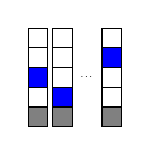
\begin{tikzpicture}[baseline={([yshift=-0.5ex]current bounding box.center)},
      scale=0.25, every node/.style={transform shape}]
      \fill[blue] (1.25*1,3) rectangle ++(1,1);
      \fill[blue] (1.25*2,2) rectangle ++(1,1);
      \fill[blue] (1.25*4,4) rectangle ++(1,1);
      \node (ellipses) at (1.25*3 + 0.5, 3 + 0.5) {\Large$\cdots$};
      \foreach \x in {1,2,4} {%
        \fill[gray] (1.25*\x,1) rectangle ++(1,1);
        \foreach \y in {1,...,5} {%
          \draw (1.25*\x,\y) rectangle ++(1,1);
        }
      }
    \end{tikzpicture}
    \quad
    \action<+->{%
      g(E) = \sum_k {(-1)}^k \binom{N}{k}\binom{N + E - kM - 1}{E - kM}
    }
  \]
\end{frame}

\begin{frame}{The Wang-Landau Algorithm}
  \centering
  \includegraphics[width=0.9\framewidth]{wanglandau-bw}
\end{frame}

\begin{frame}{The Wang-Landau Algorithm}
  \centering
  \includegraphics[width=0.9\framewidth]{wanglandau-bw-deviation}
\end{frame}

\begin{frame}{The Wang-Landau Algorithm}
  \centering
  \includegraphics[width=0.9\framewidth]{wanglandau-bw-relerror}
\end{frame}

\begin{frame}{The Wang-Landau Algorithm}
  \centering
  \includegraphics[width=0.9\framewidth]{wanglandau-bw-C}
\end{frame}

\begin{frame}{The Wang-Landau Algorithm}
  \centering
  \includegraphics[width=0.9\framewidth]{wanglandau-bw-C-relerror}
\end{frame}

\begin{frame}{Next steps}
  \begin{itemize}
    \item Connecting continuous and discrete
    \item Natural images
      \begin{itemize}
        \item Spatial information
        \item Color
        \item Stereopsis
        \item Motion
      \end{itemize}
    \item High-level features like faces
    \item Generalization
    \item Inference
  \end{itemize}
\end{frame}

\begin{frame}{Acknowledgements}
  \centering
  \includegraphics[width=1in]{nsf}
  \quad
  \includegraphics[width=1in]{rpi}
\end{frame}

\begin{frame}
  How to assign an \emph{information dimension} to the random variable $X$?
  \only<+->
  \begin{align*}
    \action<+->{X_m &= \frac{\lfloor m X \rfloor}{m} \\}
    \action<+->{d(X) &= \lim_{m \to \infty} \frac{S(X_m)}{\log m}}
  \end{align*}
  \begin{itemize}
    \item<+-> \emph{Lebesgue decomposition theorem:} $d(X)$ is the fraction of
      $P_X$ that is discrete.

    \item<+-> For a $n$-vector $X$ with finite $H(\lfloor X \rfloor)$, $0 \le d(X)
      \le n$.
  \end{itemize}
\end{frame}


\begin{frame}
  \frametitle<presentation>{References}
  \nocite{*}
  \printbibliography%
\end{frame}

\end{document}

